\chapter{Background} \label{bkgnd}

\section{Limb Imaging \& The Atmosphere}
This section provides an overview of the atmosphere, specifically the upper troposphere/lower stratosphere (UTLS) region that the LIFE instrument is designed to measure. This region is discussed in detail, with topics including the species found in both the troposphere and stratosphere, the mixing of these regions that form the UTLS region, and the need for better measurements in the future. This section will also discuss atmospheric limb remote sensing, including different methods as well as instruments that have been important to this field.

\subsection{UTLS Overview}
The atmosphere of Earth is divided into several layers, according to its thermal structure. The two lowest layers, the troposphere and stratosphere, are described here as they are most relevant to the LIFE instrument. Also described here are the main constituents of interest to LIFE: Methane (CH\textsubscript{4}), Water Vapour (H\textsubscript{2}O), Ozone (O\textsubscript{3}), and Nitrous Oxide (N\textsubscript{2}O). Finally an overview is given of the border region of these two layers, known as the UTLS, the measurement region of the LIFE instrument.

\subsubsection{Troposphere \& Stratosphere Species}
From ground level up to roughly 10 km, temperature decreases steadily. This region is known as the troposphere and its temperature is dependent on surface heating from Earth. As such, the altitude in this region increases as the temperature decreases. The upper boundary of this region is known as the tropopause, marked by a temperature minimum. This boundary is typically 10 km but is different depending on the geographic region, such as the tropics, where the boundary can be as high as 17 km~\citep{ext_utls}. This is the region where most weather occurs, and as a result it is continuously being cleaned of aerosols via cloud droplets, falling to the ground as rain. This region is also quite turbulent, leading to a generally well-mixed region of gases and aerosols. Throughout this region, the concentrations of long-lived atmospheric constituents are relatively uniform and independent of height, due to mixing caused by the turbulence~\citep{atmos_phys_and_climate}.

Above the tropopause is the stratosphere, which covers the region from roughly 15 km to 50 km, and is characterized by an increase in temperature. This temperature increase continues until the stratopause, the region between the stratosphere and mesosphere, where there is a temperature maximum. The warming in this region is due to absorption of solar radiation by the ozone layer and also causes very little mixing, which is an important difference between the stratosphere and troposphere. Unlike the troposphere, where a decrease in temperature causes turbulence, the stratosphere is relatively calm and as a result there is a less homogeneous mix of constituents in this region, such as the ozone layer~\citep{atmos_science}. Figure \ref{fig:atm_layers} shows a temperature and pressure profile of the atmosphere, with the atmospheric layers and the UTLS region of interest.

 \begin{figure}
\centering
  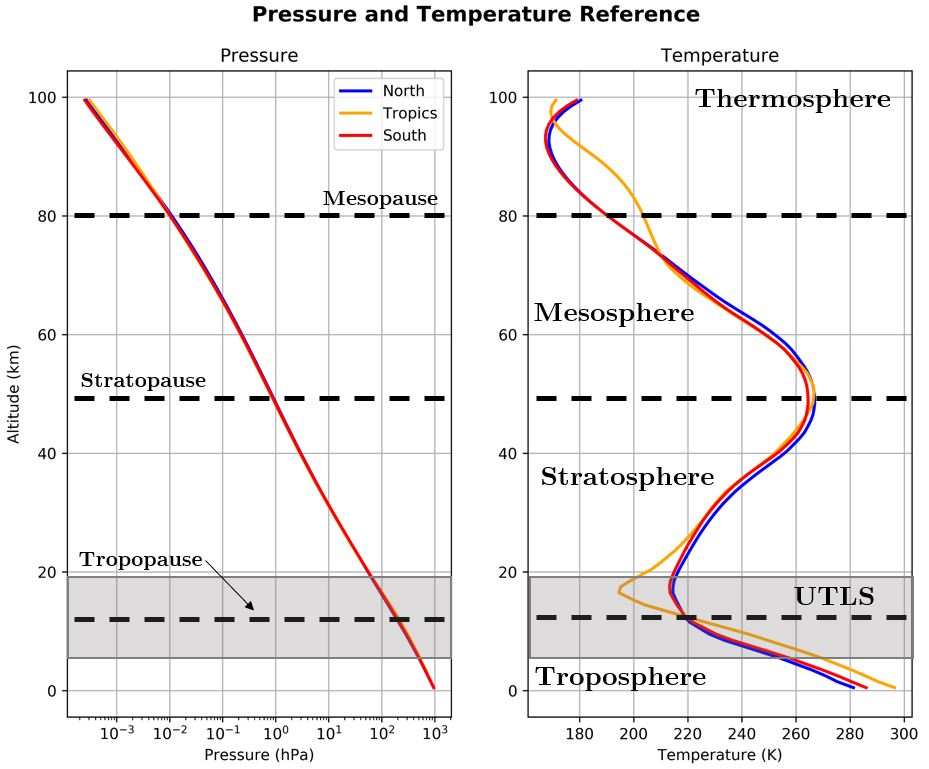
\includegraphics[width=\linewidth]{chap2_images/atmospheric_layers.JPG}
  \caption{Atmospheric layers with a typical pressure and temperature profile. The upper troposphere/lower stratosphere region is shaded grey~\citep{MSIS_model_for_profile}~\citep{ERA_interim_dataset_for_profile}.}
  \label{fig:atm_layers}
\end{figure}

 This has a large affect on one of the constituents measured by LIFE, methane (CH\textsubscript{4}). As a long-lived gas, methane can remain in the troposphere for a long period and become well-mixed. If it travels upwards to the stratosphere, it will become oxidized. As a result, methane decreases steadily as altitude increases in the stratosphere. The oxidation of methane leads to water vapour, an important greenhouse gas. Methane itself also plays a major role in the atmosphere as a greenhouse gas, which has increased exponentially in the last few hundred years as a result of human activities such as farming~\citep{atmos_phys_and_climate}. 

Similar to methane, nitrous oxide (N\textsubscript{2}O) is a long-lived constituent and as such is well-mixed in the tropopause. It comes from a variety of sources, from bacterial processes to human processes of fossil fuel combustion. In the stratosphere, it decreases with altitude, disassociating into NO. NO is important to study as it can cause the destruction of ozone, and has played a role in the thinning of the ozone layer. N\textsubscript{2}O is also a greenhouse gas and plays a role in climate change~\citep{atmos_phys_and_climate}.

Ozone (O\textsubscript{3}) is an atmospheric species mainly concentrated in the stratosphere, in the ozone layer. Below the stratosphere, it is quickly destroyed through oxidation or absorbed due to its water-solubility. It is important to study, as it is essential to life on Earth due to its absorption of UV radiation. As it also absorbs IR radiation, it also plays a role in climate change as a greenhouse gas~\citep{atmos_phys_and_climate}. The majority of ozone being concentrated in the lower stratosphere as the ozone layer, it is within the area of interest for the LIFE instrument.

In the low troposphere, water vapour is abundant, and is perhaps one of the most important atmospheric species to study. Due to its strong absorption of IR radiation it is an extremely important greenhouse and plays a major role in climate change. Stratospheric concentrations are much lower due to condensation at higher altitudes as temperature decreases, where it falls as rain or snow. If it does reach the stratosphere, it often dissociates to the free radical OH, which can damage to the ozone layer~\citep{atmos_phys_and_climate}. The results of these processes are measured by the LIFE instrument for study.

\subsubsection{The UTLS} \label{UTLS}
Now that the troposphere and stratosphere are described, the region that is of most interest to this thesis and the LIFE instrument is discussed: The upper troposphere/lower stratosphere region. This part of the atmosphere is roughly defined as the region $\pm$5 km around the boundary between the troposphere and stratosphere, and is important to study for a number of reasons. The tropospheric and stratospheric regions have very different processes, and as a result the boundary between these regions has a large affect on the chemistry of both. The exchange between the two is known as the \textit{stratosphere-troposphere exchange (STE)}~\citep{ext_utls}.

STE is part of the atmospheric circulation that moves air, pollutants, and other constituents from the troposphere to the stratosphere. The air movement is largely due to the surface of Earth heating the air, so it rises. As a result the convection and movement of air is strongest around the tropics, where the air is the warmest for most of the year~\citep{STE_text}. It cools in the UTLS region and moves toward the poles, where it falls again. This is an important process to study, as the movement of chemical constituents across this layer has direct effects on chemicals in the atmosphere, such as ozone. The destruction of ozone as well as the greenhouse gases that travel to the stratosphere via STE means that this process and the UTLS region have a critical role in studying climate change.

Research has shown that the STE has direct implications on atmospheric ozone, specifically the destruction of ozone in the stratosphere (the ozone layer) and an increase in tropospheric ozone. As mentioned previously, nitrous oxide can travel upwards through the stratosphere and disassociate to NO, a free radical. This can combine with ozone to form NO\textsubscript{x}, causing a thinning of the ozone layer in the stratosphere. Likewise, water vapour that rises to the stratosphere can disassociate to OH, a free radical similar to NO with the same ability to combine with ozone and cause damage to the ozone layer~\citep{WMO_ozone}. Water vapour and ozone are particularly sensitive to the rise and fall of air in this region due to their steep gradients in both regions (the water vapour nearer to Earth and the concentrated ozone layer)~\citep{GLORIA_objectives}. As air travels downwards via STE, it carries many of the pollutants that can affect the ozone layer, but can carry ozone into the troposphere as well. Ozone in the troposphere can have large affects on both air quality and climate change. Thus, STE plays a major role in climate change, as greenhouse gases are moved between these two layers where they have different effects~\citep{STE_text}~\citep{UTLS_STE}.

Due to the impact of chemical exchanges between the tropospheric and stratospheric layers, variability and changes to the UTLS are important in studying climate change. Changes to greenhouse gases such as ozone or water vapour in either of these regions have significant effects on chemical balance and IR absorption, leading to climate change~\citep{climate_change_2007}. In addition to this, the temperature minimum in the tropopause causes the region to be a key part of IR radiation escaping from the tropopause to space, further effecting surface climate and the climate feedback system~\citep{ext_utls}. It is clear that this region must be adequately measured to further research climate change.

These process have been measured and studied, but not in depth due to a lack of high temporal and spatial resolution measurements. Simulations and models have been created of this region, but there is a large amount of uncertainty. Some models have shown that with even small uncertainties in the exchange and processes of trace gases in the UTLS region, there is a significant effect on estimated concentrations of species such as ozone and water vapour. As a result, the radiative effects that are to be studied are highly uncertain. Measurements must be improved of trace gases and constituents in the UTLS to fix this issue. A major instrument in this area, MIPAS (Michelson Interferometer for Passive Atmospheric Sounding), took measurements from a satellite platform but with low spatial resolution. There is a gap in trace gas measurements in the UTLS that would better inform simulations of the region. The GLORIA (Gimballed Limb Observer for Radiance Imaging of the Atmosphere) instrument was the first to provide insight into this region with multiple two and three dimensional measurements with high spatial resolution~\citep{GLORIA_objectives}. LIFE is designed to follow in the GLORIA instrument footsteps in measuring this region using similar limb imaging methods via Fourier transform spectrometer. Both the GLORIA and MIPAS instruments and their objectives are described in Section \ref{instruments} as forerunners to the LIFE project. GLORIA, MIPAS, and LIFE all use limb-emission imaging to take measurements; an overview of limb imaging is provided in the section below.

\subsection{Techniques} \label{techniques}
There are many atmospheric measuring techniques, but can initially be split into two groups: passive and active sensing. Active sensing techniques involve emitting high-energy radiation and detecting its reflection to perform measurements, such as LIDAR (LIght Detection And Ranging) instruments. However, most instruments that measure in the troposphere/stratosphere region that is of interest are passive, from balloon-borne or satellite-borne instruments. Passive instruments can be further split into two groups: nadir-sounding and limb-sounding. Nadir-sounding instruments have downwards pointing geometry, and are useful for tropospheric measurements that have a high horizontal resolution. Limb-sounders look tangentially through the atmosphere, or the \textit{limb}. This method is useful for stratospheric measurements, where the constituents are less dense; with the long ray path of this method, the lower troposphere may saturate measurements due to cloud cover. This method can also provide good vertical resolution, depending on the instrument~\citep{SPARC}. An example of limb-sounding is shown in Figure \ref{fig:limb_emission_geometry}. Depending on what the instrument is scanning through the atmosphere, limb measurements are classified into four major groups: solar occultation, stellar occultation, limb scattering, and limb emission.

 \begin{figure}
\centering
  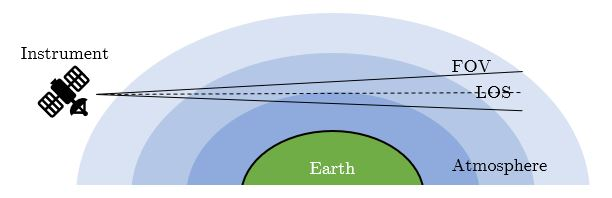
\includegraphics{chap2_images/Limb_emission_geometry_example.JPG}
  \caption{Limb emission observation example. For solar or stellar occultation, the sun or a star would be at the end of the LOS, respectively.}
  \label{fig:limb_emission_geometry}
\end{figure}

\subsubsection{Solar \& Stellar Occultation}
Solar occultation measurements are made by looking through the atmospheric limb at the sun. The radiance emitted by the sun and attenuated by the atmosphere through absorption or scattering is measured. This method allows for altitude resolved measurements as the satellite orbits the Earth~\citep{SPARC}. SAGE II (Stratospheric Aerosol and Gas Experiment), a solar occultation measurement taken as an example, begins taking measurements at a tangent height of 150 km, and continues until the sun is obscured by clouds or is below the horizon. This particular approach for SAGE II worked well as at a height of 150 km there is very little attenuation, allowing a self calibration process at lower tangent heights against 150 km~\citep{SAGEII_solar_occultation}. An issue with this method is the lack of freedom in measurement geometry, as the position of the sun and the satellite orbit defines its measurements. This leads to reduced data density compared to emission-sounding instruments, as the instrument can only take images at orbital sunrise or sunset~\citep{SPARC}. In the case of SAGE II, it took measurements 30 times per day, 15 per sunrise and sunset. Through a number of orbits, this eventually leads to global coverage~\citep{SAGEII_solar_occultation}. However, although the data density is lower than other options, the solar signal is much stronger than emission or scattering imaging, and allows for high precision measurements. Measurements from solar occultation are usually in the UV to mid-IR wavelength range~\citep{SPARC}. Some instrument examples of this method include the ACE-FTS (Atmospheric Chemistry Experiment - Fourier Transform Spectrometer) and SAGE I, II and III instruments, which primarily examined ozone but have also measured other species such as water vapour and nitrogen dioxide in the case of SAGE III~\citep{ACE_FTS}~\citep{SAGEI_and_II}~\citep{SAGE_III}.

Stellar occultation is similar to solar occultation, except the radiance from stars is measured instead. The advantage of this method over solar occultation is the greater data density that can be achieved as there is a larger time period for measuring stellar radiance over solar radiance. This method can be used during both daytime and nighttime for higher data density, but daytime measurements are typically of lower quality as the signal caused by the sun can interfere with the stellar measurements~\citep{SPARC}. The GOMOS (Global Ozone Monitoring by Occultation of Stars) instrument is an example of a stellar occultation instrument, which measures a number of species but mainly ozone. The good global coverage and measurement time of stellar occultation allows GOMOS to take 400-600 occultation measurements in 24 hours, with data being taken in both daytime and nighttime~\citep{GOMOS_stellar_occulation}. This instrument, and most similar stellar occultation instruments, measure in the spectral range shorter than 1\textmu m due to thermal emission interference at longer wavelengths~\citep{SPARC}.

\subsubsection{Limb Scattering}
Another method of limb-sounding is to measure scattered photons from the sun. These photons are scattered into the FOV of the instrument, which provides information on the atmosphere either by the scattering itself or the absorption of photons through the atmosphere. The requirement for this method is that measurements must be taken in the daytime, since the sun is the source~\citep{SPARC}. An example of limb scattering is OSIRIS (Optical Spectrograph and InfraRed Imaging System), which was the first instrument to routinely gather ozone retrieval measurements~\citep{OSIRIS}. Other examples of limb scattering measurements are the SCIAMACHY (SCanning Imaging Absorption SpectroMeter for Atmospheric CHartographY) instrument, which observes photons scattered by nitrogen, oxygen, and other aerosols, and the SME instrument which measures ozone~\citep{SCIAMACHY_limb_scattering}~\citep{SME}.

\subsubsection{Limb Emission}
Limb emission instruments measure radiation emitted by the atmosphere, either thermally or photochemically, along the instrument line of sight (LOS). These are generally low signal level emissions, but can be measured with sensitive instruments. Variation of the LOS or a wide FOV allows altitude-resolved measurements from clouds in the troposphere up through the thermosphere. Limb emission focuses on the 2.5\textmu m wavelength region and above, as the Planck function is very low for wavelengths any shorter than this at the temperatures expected in the atmosphere. In this range atmospheric scattering will not have an effect on measurements. However, a large advantage to this method is the ability to take measurements both at day and night. As no direct illumination source is needed as in other methods, a very dense spatial coverage can be created if the instrument is on a satellite platform. The viewing angle can also be freely chosen as long as it does not directly look at the sun, but this angle must be known to a high degree of accuracy to prevent any propagation errors in the data~\citep{IR_limb_emission_measurements}~\citep{SPARC}.

Many early instruments to use this method were low-Earth-orbit instruments that were used to measure vertically resolved profiles of temperature, trace gases, clouds, and aerosols. With many temperature measurements and three-dimensional chemical structure information, these instruments immensely improved understanding of the middle atmosphere region. Instruments such as CRISTA (Cryogenic Infrared Spectrometers and Telescopes for the Atmosphere) focused on high-spatial resolution, and MIPAS followed with a focus on high spectral resolution to acquire the most complete set of data in the stratosphere over its decade on-board the ESA satellite Envisat~\cite{GLORIA_objectives}.

This method is of most interest to this thesis, as it is the method used by the LIFE instrument, as well as instruments described below that paved the way for LIFE such as MIPAS and GLORIA. This is chosen for these instruments due to the vertical resolution given by a limb-viewing geometry, as well as the trace gases and constituents that are better detected with limb-viewing thermal emission.

\subsection{Instruments} \label{instruments} 
There have been a number of instruments that have taken measurements in the UTLS region using a number of different imaging methods, as described in Section \ref{techniques}. However, out of these instruments, two in particular are similar to the LIFE instrument: MIPAS, developed at the University of Karlsruhe in Germany and launched in 2002 aboard the Envisat from the European Space Agency~\citep{MIPAS_instrument}, and GLORIA, also developed at the University of Karlsruhe and was flown multiple times on aircraft in the last 10 years~\citep{GLORIA_concept}. These instruments, like LIFE, are thermal emission instruments that use a Fourier transform spectrometer to image the atmosphere. As these instruments lay the foundation for the development of the LIFE instrument, the background and description of each of these instruments are given in this section.

\subsubsection{MIPAS}
A key early instrument in the measurement of limb emissions from space is the Michelson Interferometer for Passive Atmospheric Sounding (MIPAS). It was the first instrument to use a high resolution FTS for limb emission measurements on-board a satellite. This FTS was used to measure profiles of numerous atmospheric species: H\textsubscript{2}O, O\textsubscript{3}, CH\textsubscript{4}, N\textsubscript{2}O, HNO\textsubscript{3}, and NO\textsubscript{2}, as well as aerosols such as ice clouds. To capture the radiances of these species, MIPAS had a number of spectral ranges: 685-970 cm\textsuperscript{-1}, 1020-1170 cm\textsuperscript{-1}, 1215-1500 cm\textsuperscript{-1}, 1570-750 cm\textsuperscript{-1}, and 1820-2410 cm\textsuperscript{-1}. This spectral range is used as the atmospheric signals are higher in this range to maximize the Planck function around 10\textmu m at atmospheric temperatures~\citep{MIPAS_instrument}~\citep{MIPAS_conference}.

The main purpose of this instrument is to study dynamics and chemistry from the upper troposphere region to the lower thermosphere. Studying this area of the atmosphere stems from a number of scientific objectives. The first objective is the study of stratospheric chemistry, and specifically the ozone layer. This includes studying the effect of cooling in this region, as a result of ozone depletion and increasing carbon dioxide. Another objective is studying the STE, an important part of the UTLS region as described in Section \ref{UTLS}. Finally, similar to LIFE, an objective was studying various constituents in the upper troposphere, such as water vapour, for its great importance in climate change. This also includes NO\textsubscript{x} gases and gases moving down from the stratosphere such as ozone. Overall, one of the main goals of this instrument is to observe global changes in the composition of the atmosphere resulting from pollution and other man-made effects throughout its multi-year lifetime~\citep{MIPAS_instrument}.

MIPAS, and similar instruments such as the Atmospheric Chemistry Experiment Fourier Transform Spectrometer (ACE-FTS), utilize Fourier transform spectrometers in their measurements~\citep{SPARC}~\citep{ACE_conference}. However, a limitation of these instruments is that they are not imaging instruments; they have only a single detector pixel. Limb scanning must be used to cover the atmospheric limb, where the instrument moves the line of sight upwards and downwards. However, new and larger data storage and transfer techniques have led to the usage of the imaging Fourier Transform Spectrometer (IFTS), which generates a high amount of data. With a larger throughput, more pixels can be used to create a much wider FOV that covers the atmospheric limb, thus not needing any movement of the instrument. The first instrument to demonstrate the imaging FTS concept for atmospheric measurements is a second generation MIPAS instrument, the GLORIA instrument~\citep{GLORIA_concept}.

\subsubsection{GLORIA}
The Gimballed Limb Observer for Radiance Imaging in the Atmosphere (GLORIA) instrument is an airborne limb imaging instrument operating in the thermal infrared region, similar in concept to MIPAS and LIFE. The instrument was designed to take advantage of two dimensional infrared detector array technology that had become available in the last few decades. This allowed the instrument to overcome one of the primary issues with MIPAS, which was the scanning of the atmosphere with one pixel. This two dimensional array also means that three dimensional measurements can be made when using an aircraft and tomographic techniques. This large array was designed to work with an IFTS to provide very high spectral coverage, sensitivity and spectral resolution that no instrument before has managed to achieve. This followed from a need to take measurements in the region of the UTLS where mission objectives similar to MIPAS and LIFE are to address the gap in data from satellite and airborne instruments of phenomena in this region. This includes the STE, pollutant transport across the region and ozone in both the ozone layer and the upper troposphere. Further mission objectives include measurements of gravity wave propagation in the tropopause, requiring three-dimensional observations of trace gases and temperatures with a high vertical resolution and moderate horizontal resolution~\citep{GLORIA_concept}~\citep{GLORIA_objectives}. 

The instrument consists of a cooled imaging Fourier transform spectrometer with a cryogenic Mercury-Cadmium-Telluride (MCT) two-dimensional detector array for detection of infrared radiation. This is mounted on a gimbal that is attached to a research aircraft, allowing for free viewing where needed. For calibration, two blackbodies are also mounted on-board, along with a deep-space view for further calibration~\citep{GLORIA_concept}. GLORIA operates in the region of  780 cm\textsuperscript{-1} to 1400 cm\textsuperscript{-1}, making the detector sensitive to numerous species, including H\textsubscript{2}O, O\textsubscript{3}, CCl\textsubscript{4}, HNO\textsubscript{3}, ClONO\textsubscript{2}, HO\textsubscript{2}NO\textsubscript{2}, and chloro-flourocarbons (CFCs). The instrument will image from 4 km up to the height of the aircraft, and with its high vertical resolution be able to measure steep gradients in trace gases and characteristics of clouds in this region to help meet its mission objectives. ~\citep{GLORIA_PhD}~\citep{GLORIA_objectives}.

GLORIA can also operate in two different measurements modes: chemistry mode (CM) and dynamics mode (DM). In chemistry mode, spectral resolution is maximized to increase the number of retrieved gas species with a reasonable spatial sampling. Dynamics mode is used to be able to take three dimensional data of species and temperature, with the disadvantage being a lowered spectral resolution. The instrument used both of these measuring modes successfully on multiple airborne flights on the German High Altitude and Long Range research aircraft (HALO)~\citep{GLORIA_concept}. 

\section{Thermal Design}
The thermal environment of a balloon-borne atmospheric instrument is complex, as it goes through a number of stages: It must stay cool in the lab environment, be able to survive ascent through various temperature gradients, thermally remain steady throughout the measurement window in the float portion of the flight, be able to survive the thermal radiation of sunlight later in the flight, and survive the descent. The thermal design of the LIFE instrument, and similar thermal imaging instruments, are of particular importance as the thermal signature of the instrument can have a large affect on the noise of the measurements. As a result of complexity and importance of this problem, the thermal design (with the interconnected mechanical design) of the LIFE instrument is one of the main components of this thesis. 

In this section, a background of thermal design is given that is relevant for thermal imaging balloon borne instruments. Central to thermal design is heat transfer, or the thermal phenomena of radiation, conduction and convection. These are described in detail. Following, the balloon environment is described in more detail, with an example from a previous instrument flight. Self-emission, very important for the design of a thermal emission imaging instrument, is discussed. Thermal control methods that are considered when designing an instrument for extreme temperatures are discussed after. The thermal designs of MIPAS and GLORIA, which have similar thermal requirements to LIFE as thermal imaging instruments, are described at the end of this section.

\subsection{Heat Transfer}\label{heat_transfer}
Heat transfer is a very broad topic, covering theoretical physics and engineering physics as well as engineering design. It is covered in many articles, journals, and textbooks. Only a high level of background is given here to help understand the thermal phenomena important to thermal analysis, particularly for a balloon-borne atmospheric instrument. At its most basic, heat transfer is dependent on the Second Law of Thermodynamics: \textit{Heat flows from a hot body to a cold body, increasing the entropy of a closed system}. Heat is a form of measurable energy, discussed in terms of the temperature of bodies. Heat of a material may be related to a number of phenomena, such as atomic or molecular motion of a material, or to electromagnetic radiation~\citep{Heat_Transfer_telescope}.

Heat transfer occurs in three different ways: Radiation, conduction, and convection. These control the flow of heat energy through an object, and each play a different role; radiation emits heat from an object into space, not requiring any outer medium. Conduction defines how heat travels through an object, or a connection between two objects, and convection describes heat moving from an object to a surrounding fluid medium. Each of these phenomena are described in detail here.

\subsubsection{Conduction}\label{Conduction_sec}
Thermal conduction is the process of heat transfer across solids. This can be done through molecules, atoms, electrons or photons carrying energy. As mentioned previously, the second law of thermodynamics states that heat will always flow from a hot body to a cold body~\citep{Heat_Transfer_Basics}. As a result, thermal conduction will occur in any material where a temperature gradient exists, and as such can play a very important role in thermal design where heat must be moved away from components generating high heat power.

When there is a temperature gradient in a material, there will be heat flux, \textit{q}. Heat flux, also known as thermal flux, is the flow of energy per unit area. Most often in units of W/m\textsuperscript{2}, heat flux is used to calculate how much heat is traveling through a medium. Through a body, heat flux is described by \textit{Fourier’s Conduction Law}, shown in Equation \ref{FC_law}.
\begin{equation} \label{FC_law}
    \bm{q}(T) = -k\nabla T
\end{equation}

Here \textit{k} is the thermal conductivity of the material and $\nabla$\textit{T} is the spacial temperature gradient~\citep{heat_transfer_textbook}. This equation can be used to develop the equation for the heat through a surface area:
\begin{equation} \label{heat_rate_conduction}
    Q = \int_{A}q_ndA
\end{equation}
Here, $q_n$ is the same heat flux vector as above, but normal to the surface~\citep{Heat_Transfer_Basics}.

The thermal conductivity is an important aspect of this equation. For an anisotropic material, the conductivity is a tensor and the temperature gradient forms a vector, which makes the Equation \ref{heat_rate_conduction} very difficult to solve. For most designs and technical applications, especially as most materials are isotropic at a macroscopic level, the thermal conductivity can be taken as a mean value. The thermal conductivity is dependent on the material and has units of W/mK~\citep{heat_transfer_textbook}~\citep{FEA_SW}. The design control for the conduction of heat relies on \textit{k}, thus the material chosen. 
% transient conduction could be described here if some more background is needed but probably not necessary.

Another aspect of thermal conduction that must be considered for thermal simulations are boundaries. In many cases, contact between two parts can be simplified to 'bonded' or 'insulated', meaning either full contact as if they were one part, or completely disconnected, respectively. Often parts can be thermally connected using a thermal paste, increasing the contact by as much as 75\%~\citep{Heat_Transfer_Resistance}, making the bonded simplification reasonably accurate. However, in the cases of junctions with a large surface area where thermal paste is not applied, a more careful examination is needed. Instead of a smooth temperature gradient across the connection, there can be a discontinuity, due to the surfaces not being perfectly connected. This is known as \textit{thermal contact resistance}. 

Thermal contact resistance is largely a result of surface roughness. At a joint, there are two main contributions to heat flow: Solid-to-solid conduction at points of contact between the two bodies, and the conduction through entrapped gases in the spaces between contact. Conduction happens easily through direct solid-to-solid contact, but not in gases. These gases are the major cause of thermal contact resistance, as the thermal conductivity of gases is very small compared to solids and particularly metals. This plays an even larger role in the atmospheric balloon environment, where vacuum means that there are not even gases to transfer heat, so the thermal resistance is larger~\citep{Heat_Transfer_Resistance}. 

An equation for heat conduction across a joint can be developed, leading to an equation for solving for $h_c$, known as the contact coefficient. This contact coefficient determines how well heat flows across a joint. If the contact area of a junction is denoted by $A_c$ and the void area by $A_v$, the equation for heat flow across a joint is given by Equation \ref{heat_flow_joint}. % could provide a bit more background on this equation if needed

\begin{equation}\label{heat_flow_joint}
    q = \frac{T_1 - T_2}{\frac{L_g}{2k_1A_c}+\frac{L_g}{2k_2A_c}}+k_fA_v\frac{T_1-T_2}{L_g} = \frac{T_1-T_2}{\frac{1}{h_cA}}
\end{equation}

In this equation $T_1$ is the temperature of the first body, $T_2$ is the temperature of the second body, $k_1$ is the thermal conductivity of the first body, $k_2$ is the thermal conductivity of the second body, $L_g$ is the thickness of the void space between bodies, $k_f$ is the thermal conductivity of the fluid filling this void space, and $A$ is the total area that should be in contact between the two bodies (at a macro scale). $1/h_cA$ is the thermal contact resistance. The left side of this equation is the heat flow due to the solid conduction plus the heat flow due to the fluid conduction, and the right side is the full heat flow~\citep{Heat_Transfer_Resistance}. From these equations the contact coefficient $h_c$ can be solved for to obtain Equation \ref{contact_coeff_eq}.

\begin{equation}\label{contact_coeff_eq}
    h_c = \frac{1}{L_g}\left( \frac{A_c}{A}\frac{2k_1k_2}{k_1+k_2}+\frac{A_v}{A}k_f \right)
\end{equation}

This equation can be slightly simplified for a balloon environment (vacuum, hence $k_f$ = 0) as well as the conductivity of the materials being equal, shown in Equation \ref{contact_coeff_eq_simplified}.

\begin{equation}\label{contact_coeff_eq_simplified}
    h_c = \frac{A_c}{A}\frac{k}{L_g}
\end{equation}

From the above equation, it appears that the contact coefficient could be calculated rather simply. However, it is extremely difficult to find an accurate value for either the contact area or the size of the gap between parts. There is no theory or even empirical evidence that is reliable. This is to be expected due to the high amount of unknowns involved, mainly direct surface area contact of a material, which cannot be accurately quantified~\citep{Heat_Transfer_Resistance}~\citep{stephane_thermal_contact}. The most accurate way of finding this is often through finding a rough estimate, building, and testing the joint in a thermal vacuum chamber. This was done with the LIFE instrument. Further analysis for the thermal resistance in the case of LIFE is described in Section \ref{final_pre_flight_sims}.

In a vacuum environment, conduction is one of two forms of heat transfer, due to the lack of convection. Thus it is more important to take this into account for any electronics or instruments operating in a vacuum environment, such as an atmospheric instrument. Heat must be able to flow between parts in order to dump heat properly, or they will overheat. A good contact between all parts is essential to an operational instrument. The only other method of heat transfer in this environment is through radiation. 

\subsubsection{Radiation}\label{radiation_sec}
Thermal radiation is heat transfer carried by electromagnetic waves, in the wavelength range of 0.1-1000 \textmu m. As electromagnetic waves do not require any medium to travel, neither does thermal radiation. As such, radiation occurs in vacuum, and with the absence of convection in a vacuum due to the need of a medium, it plays an important role in these environments~\citep{Heat_Transfer_Basics}. Radiation can often be neglected, but in a vacuum environment and at higher temperatures it must be included in the thermal design process.

The intensity of the energy flux radiated from the body is dependent on the temperature of the surface, and increases with temperature. In addition to temperature, the radiation from a surface depends on its emissivity {\textepsilon}, which is a characteristic of the material or its coating. A blackbody is an object that has a very high emissivity, and an ideal blackbody has an emissivity of 1, meaning that it can emit electromagnetic waves at any temperature with maximum intensity. For a typical blackbody, the emissivity is equal to its absorptivity {\textalpha}, which is how much radiation is absorbed by the surface. This is why they are known as blackbodies; for comparison, whitebodies would absorb no radiation, with an absorptivity of zero. In reality, all surfaces and materials are somewhere in between these two extremes, and are known as greybodies~\citep{Heat_Transfer_Basics}~\citep{heat_transfer_textbook}. The material or coating, and thus the emissivity, must be taken into account in thermal design and is a method of controlling the thermal design to allow the object to emit more or less heat.

It is possible to make an almost perfect blackbody ({\textepsilon} {\textgreater} 0.99), which is often used for calibrating instruments to precise temperatures. A common device is known as a \textit{hohlraum}, German for "hollow space". It is a hollow cylinder or sphere with an opening, with an interior coated with an extremely high emissivity black coating. The interior of the hohlraum is designed to have some sort of rough surface (such as pyramidal structures). With this setup, radiation enters the opening and is almost entirely absorbed by the coating. The parts that do not get absorbed are reflected from the rough surface to another part of the cylinder, where it is absorbed further. In this way, almost all radiation is absorbed, allowing the temperature of the surface to be very clearly and accurately seen by an infrared detector~\citep{Heat_Transfer_Basics}~\citep{heat_transfer_textbook}. An example diagram of this device can be seen in Figure \ref{fig:blackbody_example}. This sort of device plays an important role in LIFE and similar thermal imaging instruments for calibrating the detector at various temperatures.

 \begin{figure}
\centering
  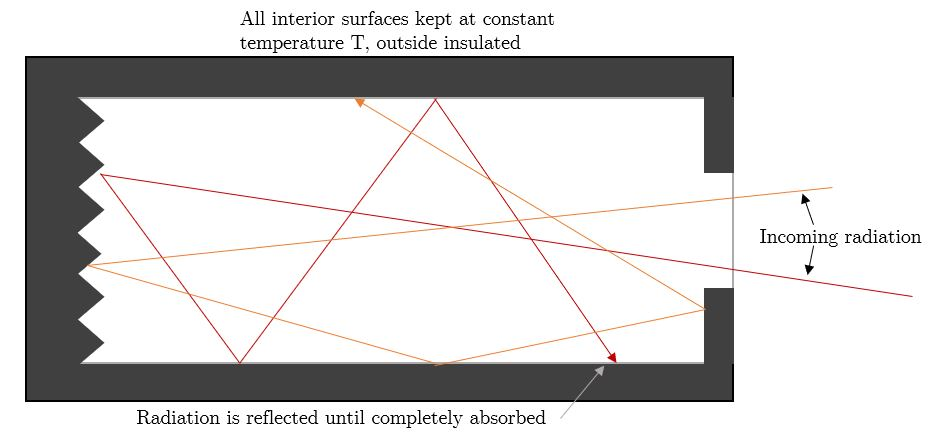
\includegraphics[width=\linewidth]{chap2_images/blackbody_example.JPG}
  \caption{Example of a near-perfect blackbody, known as a \textit{hohlraum}. This is a cross-section of a cylindrical system similar to what is used on the LIFE instrument.}
  \label{fig:blackbody_example}
\end{figure}

The spectral intensity of the radiation emitted from an ideal blackbody surface can be calculated, and is given by Planck's radiation law, in Equation \ref{plancks_law}.

\begin{equation}\label{plancks_law}
    L(\lambda) = \frac{2hc^2}{\lambda^5}\cdot\frac{1}{e^{(\frac{hc}{\lambda k_B T})}-1}
\end{equation}

Here $h$ is Planck's constant, $c$ is the speed of light, $\lambda$ is the wavelength of incoming radiation, $k_B$ is the Boltzmann constant ($1.38\cdot 10^{-23}$ J/K), and T is the blackbody temperature~\citep{Heat_Transfer_Basics}. This equation gives the Planck curve of the radiation emitted from an object, and is important to the calibration of thermal imaging instruments. This equation is used when calculating spectral radiances for the LIFE detector responsivity, discussed in Chapter \ref{detector}. Its units are $\mathrm{Wm^{-2}sr^{-1}}$.

The energy emitted from the blackbody surface reaches a theoretical maximum due to the emissivity of 1, and this maximum is given by the Stefan-Boltzmann Law. This law is calculated by the integration of wavelength of Equation \ref{plancks_law} from zero to infinite wavelength~\citep{Heat_Transfer_Basics}. This equation, which gives the flux of energy radiation for a blackbody $q_b$ in $\mathrm{W/m^2}$, is shown in Equation \ref{SB_law}.

\begin{equation} \label{SB_law}
    q_b(T) = \sigma T^{4}
\end{equation}

where the Stefan-Boltzmann constant, \textsigma, is $5.67\cdot10^8$ W/m\textsuperscript{2}K\textsuperscript{4} (equal to all constants left from integration), {\textepsilon} is the emissivity of the surface, and \textit{T} is the absolute temperature. For non-blackbodies, the heat flux emitted is the blackbody heat flux multiplied by the emissivity. The total energy radiated can also be shown by multiplying by the area, $A$. Thus the Stefan-Boltzmann Law equation for general surfaces is given below as Equation \ref{SB_law_general}~\citep{Heat_Transfer_Basics}.

\begin{equation} \label{SB_law_general}
    q(T) = \epsilon \sigma T^{4} A
\end{equation}

In most situations, radiation from one surface will intersect with objects in its surroundings. Equation \ref{SB_law} and \ref{SB_law_general} both assume the radiated energy is absorbed by the medium or far surroundings, thus having no affect on the emitting object. In reality, an object emitting energy will have energy emitted to it by a nearby body. The Stefan-Boltzmann Law must be altered for this scenario.

The simplest form of this problem is that all radiation from a blackbody object, say object 1, is absorbed by another blackbody object, say object 2. Likewise, all radiation from object 2 is radiated to object 1 and absorbed. The net heat transferred from object 1 to object 2, known as $Q_{net}$, is the difference of the radiation from object 1 to object 2 and the radiation from object 2 to 1~\citep{heat_transfer_textbook}. This is shown in Equation \ref{SB_surroundings}.

\begin{equation}\label{SB_surroundings}
    Q_{net} = A_1 q_b (T_1) - A_1 q_b (T_2) = A_1 \sigma (T_1^4 - T_2^4)
\end{equation}

Here, $T_1$ is the temperature of the first object, $T_2$ is the temperature of the second object, $A_1$ is the area of the first object, $q_b$ is the heat flux emitted from the first object, and {\textsigma} is the Stefan-Boltzmann constant. In many situations, this is often good enough. However, the more realistic scenario is that the objects see other objects too, and not all radiation from one object is absorbed by a single other object. To account for this, a view factor $F_{1-2}$ must be included in the equation. Essentially, this view factor is how well the surface 'sees' the other surface~\citep{heat_transfer_textbook}~\citep{FEA_SW}. Assuming two small areas $A_1$ and $A_2$, the view factor can be calculated using Equation \ref{view_factor}.

\begin{equation}\label{view_factor}
    F_{1-2} = \frac{1}{A_1} \Int_{A_1} \Int_{A_2} \frac{cos \theta_1 cos \theta_2}{\pi R_{1-2}^2} \,dA_1\,dA_2
\end{equation}

Here, $\theta_1$ and $\theta_2$ are the angles between the unit normal of each area, and $R_{1-2}$ is the line connecting the two areas. This equation is inserted into Equation \ref{SB_surroundings} with the surface emissivity to create Lambert's Law, giving the heat flow rate between two gray diffuse surfaces, shown in Equation \ref{Lamberts_Law}.

\begin{equation}\label{Lamberts_Law}
    Q_{net} = \epsilon A_1 \sigma F_{1-2} (T_1^4 - T_2^4)
\end{equation}

This question assumes the surfaces have the same emissivity. If they have different values, this equation becomes more complex.

As discussed in Section \ref{FEA}, a thermal simulation often breaks a surface into many small surfaces to be able to run the simulation. As such, this equation, and particularly Equation \ref{view_factor}, must be solved hundreds of thousands of times for each simulation. As such, it requires major computational power to run simulations that include surface-to-surface emissivity. For the purpose of saving time in simulations, this is often approximated by estimating the ambient temperature an object will see when radiating, along with an estimated view factor, and changing if necessary. This will make simulations less accurate but many more simulations are able to be run, so these settings can be iterated with trial and error until they are deemed accurate.

 In relation to the thermal design, the two main variables that can be altered when running simulations and testing designs are the surface area and emissivity. Choosing the right material to either maintain or emit heat through radiation to stop freezing or overheating, as well as designing to allow heat to be dumped to less heat-sensitive parts of the instrument through conductivity, are critical parts of thermal design.

\subsubsection{Convection}\label{convection_sec}
For most of the LIFE thermal simulations, convection does not play a part. This is because at the altitude LIFE floats at, roughly 30-35 km, there is essentially a vacuum. There is no medium for convection to act in, thus it is not considered in the simulations. However, the ascent from the ground through the tropopause to the float altitude was simulated, and convection still played a part in this aspect of the flight; especially through the cold tropopause. As such, and as it often plays an extremely important role in thermal design, it is discussed here. However, convection is more complex than the previous two methods of heat transfer, due to the involvement of fluid dynamics. It will only be discussed here at a high level.

Convection occurs when a cool fluid flows past a warm body, carrying away heat. The air closest to the body forms a boundary layer, where the moving air is slow. In this region, conduction moves heat from the body to the fluid. The fluid then carries this heat away downstream, and in this way the heat from the body is constantly being stripped away~\citep{heat_transfer_textbook}. Cooling through the convective process can be described by a simple formula, originally developed by Isaac Newton. If the energy of a body is constantly replenished, and the temperature of the oncoming fluid remains constant, the heat removed by the convective fluid is proportional to the difference of the object temperature and the fluid temperature. This equation can be written to solve for the heat flux from the object, shown in Equation \ref{newtons_equation}.

\begin{equation}\label{newtons_equation}
    q = \bar{h}(T_{body} - T_{\infty})
\end{equation}

This is known as Newton's law of cooling in the steady state, and here $T_{body}$ is the temperature of the body, $T_{\infty}$ is the temperature of the fluid, and $\bar{h}$ is the average heat transfer coefficient. The units of $q$ are W/m\textsuperscript{2} as usual with heat flux, so the units of $\bar{h}$ are W/m\textsuperscript{2}K~\citep{heat_transfer_textbook}.

An issue with simulating convection is the heat transfer coefficient; it is very difficult to find an accurate value for $\bar{h}$, as it is dependent on a large number of variables. Firstly, it is sometimes dependent on $(T_{body} - T_{\infty})$, or $\Delta T$. This dependence is based on if the fluid is forced past a body, known as \textit{forced convection}, or if the fluid is still, known as \textit{free} or \textit{natural convection}. If $\Delta T$ is small, there is a negligible dependence, but can have a large effect (up to $\Delta T^2$) if the temperature difference is large. Natural convection, which behaves differently than forced convection as it is more dependent on the heat from the object causing air to rise (and thus bringing colder air back down against the object, causing a cycle). This leads to a small dependence on $\Delta T$, on the order of $\Delta T^{1/3}$. In addition to these dependencies, it is dependent on pressure through the Reynolds number (used through fluid turbulence calculations near the object surface), the material and its conductivity, and the material surface and shape~\citep{heat_transfer_textbook}.

Due to this large variety of unknowns, it is quite complex to calculate the heat transfer coefficient, even for just one scenario, which can change quickly. Calculated values of $\bar{h}$ for one scenario (for forced convection over an aluminum surface, for example) can vary over 6 orders of magnitude, causing massive changes to the simulation~\citep{heat_transfer_textbook}. It is recognized that this is one of the largest unknowns with the thermal design and simulations as a result.

If a heat transfer coefficient is known, Equation \ref{newtons_equation} can estimate the heat flux reasonably well, enough for LIFE thermal simulation purposes. Much theory surrounding convection is solving for the heat transfer coefficient, and even then still have a large amount of error, and solving equations related to the boundary layer. For the purposes of the LIFE thermal simulations, and considering that convection plays a role in only a small portion of the flight, these equations will not be described. In the simulations, as described in Chapter \ref{postflight}, a heat transfer coefficient is chosen out of an estimated range from literature, and iterated through multiple simulations, as is often the most practical way of finding the coefficient. 

\subsection{Balloon Environment} \label{balloon_env}
Thermal design is a crucial part of atmospheric instruments, and particularly thermal imaging instruments. The thermal environment seen by these instruments varies widely, in a number of different scenarios: In the lab on the ground, during the ascent, during float, both with and without the sun. For example, when a balloon-borne instrument is travelling upwards through the tropopause, where the temperature reaches extreme temperatures as low as -80°C, the temperature of the instrument can drop very rapidly. When working with delicate thermal imaging instruments where the temperature can affect measurements, this can be catastrophic, and it is important that this is taken into account during design.

On the ground, most instruments are cooled with a combination of conduction and convection. Convection often plays a large role in the lab by using fans to cool the instrument. However, at high altitudes, the pressure is very low and can be considered vacuum. As described in Section \ref{heat_transfer}, convection requires a medium to move heat away to cooler areas. Without any fluid, heat is only transferred through conduction and radiation. Convection will play a role during ascent, as the air is still dense enough in the lower troposphere to have an affect, but decreases rapidly. This lends complexity to the thermal design, as there is little information on how the convection coefficient changes at higher altitudes. 

If the instrument is not flying overnight, the sun will have a large affect on heating at these altitudes. The solar flux is the heat transferred to an object from the sun. The atmosphere lowers this flux by attenuation, so that it is not as intense at ground level. In the lower stratosphere where the instrument will sit for the majority of its flight, the sun can be extremely intense and can heat the instrument very quickly if no shielding is provided. It should be known if the sun will be seen during the balloon flight of an instrument so it can be shielded and able to dump heat accordingly.

Due to the extreme variation in temperatures that the instrument will see from the ascent through the tropopause to the sun, it is helpful to have data on what can be expected. Data is provided from a previous atmospheric balloon-borne instrument from the University of Saskatchewan, launched from the same location as LIFE in Timmins, Ontario. This data was measured throughout the flight in August of 2018 by the National Centre for Space Studies (CNES), who operated the balloon. It is shown in Figure \ref{fig:2018_timmins_temps}, which shows temperatures for numerous sensors scattered around the balloon gondola~\citep{CATS_report}.
 
 \begin{figure}[h!]
\centering
  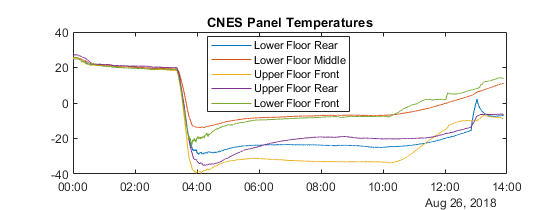
\includegraphics{chap2_images/CNES_temps_CATS_2018.png}
  \caption{High altitude balloon temperatures in °C during 2018 flight in Timmins, Ontario.}
  \label{fig:2018_timmins_temps}
\end{figure}

It can be seen in Figure \ref{fig:2018_timmins_temps} that the lowest gondola temperature reached during the flight was -40°C, while travelling through the tropopause. Of note in this region is the sharp decrease in temperature throughout this region, in a matter of minutes. The thermal shock of this temperature drop must be considered for delicate electronic components and optics. Temperatures for thermal simulation scenarios were chosen based on what was seen here, which is described further in Chapter \ref{thermal}.

Atmospheric instruments often have delicate optics or electronics, so the thermal characteristics of the instrument are a very important part of the design. Particularly for thermal imaging instruments, the optics must be carefully controlled in order to reduce the thermal radiation background, or self-emission, effect on measurements. Self-emission can lead to systematic errors in the data, as part of the data collected are thermal emission signatures from the optics rather than the atmosphere. This is gone over in further detail in Section \ref{self-emission}. Various instruments use different methods to maintain appropriate operational conditions for the instrument. The MIPAS and GLORIA thermal designs are discussed in Section \ref{GLORIA_MIPAS_thermal} for context. 

\subsection{Self-Emission}\label{self-emission}

Self-emission is an important part of limb-emission imaging instruments and must be considered in the thermal design. As limb-emission instruments measure in the infrared range to detect thermal signatures of species from emissions, they detect all thermal signatures. This will include anything that is in the path of the detector, which includes any lenses or windows in the optical system. Self-emission is known as the aspect of the measurement signal that is not from the atmospheric measurements but from elements of the instrument, usually the lenses, that are also in the path of the detector. This addition to the signal causes issues in the signal-to-noise ratio, if the temperature of the lenses as seen by the detector begins to wash out any signal of the atmosphere, and also the radiometric calibration and phase determination of the data, as this self-emission also has signal phase effects on the measurements.

The addition of the self-emission signal to the total measured signal can be shown mathematically. The signal measured by the detector can be split into three major sources: radiation from the atmosphere $S_b$ (the goal of the measurement), emission from optical components $S_o$, and emission from the beam-splitter of the FTS $S_b$~\citep{self-emission_general}. Together, these make up the total interferogram signal.

These self emission components can be calibrated out through the Revercomb method~\citep{Revercomb_method} that is used to calibrate the GLORIA measurements~\citep{gloria_self_emission}. A core assumption in this calibration process is that the temperature causing the self-emission signal is constant with time in a sample window. This leads to the requirement for many of the thermal emission imaging systems having steady temperature optics, with no gradients across lenses and very small temperature drift over the course of a sample window. MIPAS, GLORIA, and LIFE all have this requirement.

As self-emission is caused by the thermal signal of the instrument, a simple way to remove a large part of this signal is by cooling the optical system to low temperatures, greatly improving the signal to noise ratio. The MIPAS and GLORIA methods use this, as described in Section \ref{GLORIA_MIPAS_thermal}. The LIFE solution, which is a different approach, is described in Chapter \ref{thermal} of this thesis.

\subsection{Thermal Control Methods} \label{Thermal_methods} % could add radiators if necessary.
When designing an instrument with thermal requirements, it is often not possible to design to the correct temperature ranges without adding specific methods to heat or cool components of the design. There are a wide variety of methods for all applications, but this section will be just describing methods used in the LIFE instrument and similar instruments described in Section \ref{GLORIA_MIPAS_thermal}, specifically for heating, cooling, and insulation.

\subsubsection{Coolers}

While there are a vast number of types of coolers that are used in a variety of applications, there are a few that are most often used in atmospheric instrument design. Of these few, there are two that are of interest to LIFE and other instruments described in this thesis: Thermo-electric coolers (TECs) and Stirling cycle cryocoolers. Stirling coolers are used in cryogenic applications and TECs are heat pumps usually used for transferring heat from one side of a device to another in a solid-state form, and do not cool to as low of temperatures as Stirling coolers.

Thermo-electrical coolers are based upon the Peltier Effect. A simple TEC is a junction formed by semiconductors, one doped to have more holes and one doped to have more electrons. When an electric current is passed through the junction, both charge carriers move away from the junction, and there is a decrease in temperature here. Heat is thus absorbed from the environment, and carried along by electrons to the cool side. As a result a junction can be placed against a hot surface and heat will be transferred to the other side of the cooler where it can be radiated away. This devices have the advantage of being solid-state and having long lifetimes due to their simplicity, but are low-efficiency and thus are used only in specialized applications~\citep{TE_coolers}. In the LIFE instrument, a TEC is used to cool the cold blackbody surface used for detector calibration.

Stirling coolers are most often used to cool a small surface area or component to cryogenic temperatures, and operate using the Stirling cooling cycle. At its basis, it can be described as a piston system, which moves heat away from the contact surface of the cold side of the cooler and radiates on the warm side to the environment through a process of isothermal expansion and compression similar to the Carnot cycle. It is made up of a piston on the warm side, a gas compression space, a heat exchanger, a regenerator in the middle, and another heater exchanger, expansion space, and a piston on the cold side. A diagram of this system is in Figure \ref{fig:stirling_cooler}. Heat is transferred through the cooler via a fluid, and for most cryogenic applications this is either gaseous or liquid helium~\citep{cryocoolers}.

\begin{figure}
\centering
  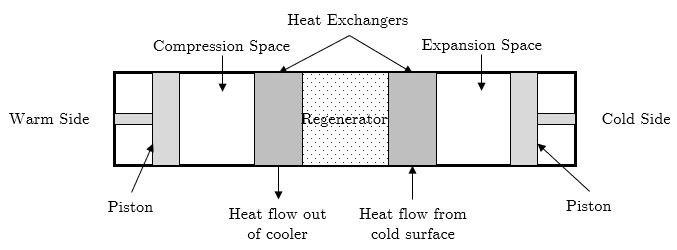
\includegraphics[width=\linewidth]{chap2_images/stirling_cooler.JPG}
  \caption{Diagram of a basic Stirling cooler.}
  \label{fig:stirling_cooler}
\end{figure}

The regenerator at the centre is a porous material that has good contact with the gas, a low flow resistance, and a high heat capacity. Its goal is to stop heat from transferring from the warm side to the cold side by absorbing heat from the fluid, so that the surface is not heated during the cooling step. The heat is transferred from the regenerator to the heat exchangers which radiate it away from the cooler~\citep{cryocoolers}.  In the ideal case, the Stirling cycle which this piston system uses to operate can be described in four steps. The first step of the cycle is shown in Figure \ref{fig:stirling_cycle_part_1}.

\begin{figure}[h]
\centering
  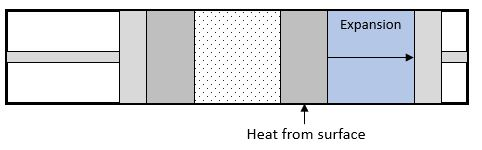
\includegraphics[width=0.8\linewidth]{chap2_images/stirling_process_cold_absorb.JPG}
  \caption{Step 1 of the Stirling cycle: isothermal expansion leading to cold absorption.}
  \label{fig:stirling_cycle_part_1}
\end{figure}

In this step, the cold piston moves to the right, causing expansion. As this expansion is ideally isothermal, heat is absorbed from the surface into the heat exchanger, which transfers it to the fluid. The next step is shown in Figure \ref{fig:stirling_cycle_part_2}.

\begin{figure}[h]
\centering
  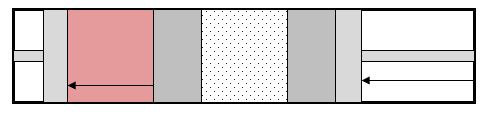
\includegraphics[width=0.8\linewidth]{chap2_images/stirling_process_cold_transfer.JPG}
  \caption{Step 2 of the Stirling cycle: Both pistons move, there is a constant volume and an increase in pressure.}
  \label{fig:stirling_cycle_part_2}
\end{figure}

Here both pistons move equally, so the volume remains constant. There is an increase in pressure so to keep temperatures constant, heat is extracted from the regenerator (it is stored here from step 4). Thus there is heat in the compression chamber from both the regenerator and the surface. It is removed from the system in step 3, shown in Figure \ref{fig:stirling_cycle_part_3}.

\begin{figure}[h]
\centering
  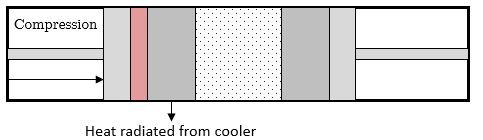
\includegraphics[width=0.8\linewidth]{chap2_images/stirling_process_heat_radiation.JPG}
  \caption{Step 3 of the Stirling cycle: isothermal compression leading to heat being radiated to surroundings.}
  \label{fig:stirling_cycle_part_3}
\end{figure}

In this step the warm side piston moves to the right, causing compression. Ideal isothermal compression leads to heat being radiated away to the environment via the warm heat exchanger. The final step leads back to step 1, shown in Figure \ref{fig:stirling_cycle_part_4}.

\begin{figure}[h]
\centering
  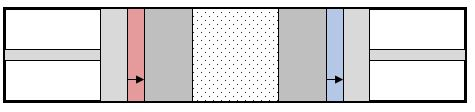
\includegraphics[width=0.8\linewidth]{chap2_images/stirling_process_heat_transfer.JPG}
  \caption{Step 4 of the Stirling cycle: Both pistons move, there is a constant volume and a drop in pressure.}
  \label{fig:stirling_cycle_part_4}
\end{figure}

In this final step, both pistons move equally once again to keep volume constant. Here there is a decrease in pressure, and to keep temperatures constant heat is trapped by the regenerator. As a result, there is little heat (what remained after radiation) in the fluid that is transferred to the expansion chamber. This means that the fluid is cool in the expansion chamber, causing more heat absorption from the surface and less warming of the surface by the fluid. The cycle then restarts~\citep{cryocoolers}. An ideal Stirling cycle pressure-volume diagram is shown in Figure \ref{fig:stirling_cycle} to summarize the steps.

\begin{figure}[h]
\centering
  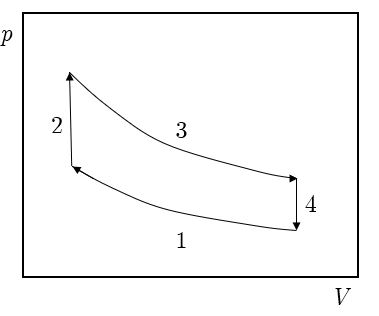
\includegraphics[width=0.5\linewidth]{chap2_images/stirling_cycle.JPG}
  \caption{An ideal pressure-volume diagram of the Stirling cycle. Non-ideally, this plot is elliptical.}
  \label{fig:stirling_cycle}
\end{figure}

Realistically, this cycle is not split into four discrete steps. Many modern Stirling coolers use a phase difference of around 90° between pistons, making a harmonic motion and can be driven by a common rotary axis. There are also more complex versions of the Stirling cooler that use a compressor and magnetic field to drive pistons~\citep{cryocoolers}. Stirling coolers are useful for cooling specific small surfaces to very low temperatures, and is used in many instruments to cool small, cryogenic instruments. It is used in LIFE to cool the infrared detector to below 70K to obtain the required sensitivity.

\subsubsection{Heaters} %feels dumb to put this into its own section, but what else is there to do?

Heaters are often needed in instruments to ensure that electronics do not freeze during operation. The most common type of heater is a high-power dissipating resistor encased in some type of conducting material. The maximum heat power that is dissipated from the heater can be chosen based on the size, and the amount of current applied to the heater can control the heat power precisely. These are most often used with a PID controller, which will raise or lower the current applied to the heater until the object being heated has reached the desired temperature~\citep{SMAD}. Components that are heated can sometimes be quite large, and if the instrument is continuously in a cold environment these heaters can draw a very large percentage of the total power of the instrument. 

\subsubsection{Insulation}

A key part of thermal design is insulating heat-sensitive components from other components where the temperature can vary rapidly or become extreme. For example, to help avoid self-emission as described previously, temperatures should be kept as steady as possible across optics. To help maintain steady temperatures even if the environmental temperatures are changing rapidly, insulation must be used. Insulators are any material that have a very low conductivity, that is $k \ll 1$. There are two insulation scenarios, one for radiation and one for conduction. A method of thermal control for each is given that pertains to this thesis.

In the case of conduction, there is a solid point of contact between two components for heat transfer, thus a solid insulator must be used. Most non-metals, typically plastics, are useful here, as they have a low conductivity. But plastics will off-gas in a vacuum environment, so cannot be used for balloon or satellite-borne instruments. Most often this is solved by using titanium. Unlike most metals, it has a very low thermal conductivity, meaning that is a good choice of material between two objects that should be isolated from each other. This is often done in the form of titanium spacers or joints, and is used on LIFE to help dissipate thermal fluctuations to the optics module.

A common insulation that is used to protect instruments from exterior heat flux, such as the sun, is multi-layer insulation (MLI). MLI blankets are the most common form of insulation for delicate instruments in extreme temperature environments. It is composed of multiple layers of low-emissivity material with a low conductivity. The material is often embossed, and made of one side aluminum and one side mylar. The embossing allows little conduction between layers due to less contact, and the mylar acts as a low conductivity spacer. Any number of layers can be used, but the effect decreases exponentially with the amount of layers~\citep{SMAD}. MLI is most often used to lessen the effects of the solar flux falling on an instrument, and as such is most often used in spacecraft. It was not considered for the LIFE instrument due to the short flight time of the instrument and flying mostly during night, but was used for insulation on MIPAS.

\subsection{Instruments} \label{GLORIA_MIPAS_thermal}
As briefly described in Section \ref{balloon_env}, the environment of balloon instruments, as well as the space environment, has many thermal implications that must be accounted for in the design. The instruments that are used for atmospheric sensing often have important thermal requirements for delicate systems, such as the Fourier Transform Spectrometers and MCT detectors. Self-emission as described in Section \ref{self-emission} also plays a very large role in the design and must be considered carefully to minimize its effect. Different instruments use different methods to meet these requirements to ensure that they survive the flight. The thermal designs of MIPAS and GLORIA, as forerunners to LIFE, are described here. Research done into the design of these instruments helped form the basis for the design of LIFE, although it was ultimately taken in a different direction.

\subsubsection{MIPAS}
MIPAS is different from GLORIA and LIFE in that it flew on-board the ESA Earth observation satellite Envisat~\citep{MIPAS_thermal}, so it is the only instrument of the three to be designed for a satellite environment. However, as the design with regards to the FTS, lens system and detector is similar to GLORIA and LIFE it is still helpful to discuss here.

The electronics have a relatively small required temperature range at 273-313K. However, operating at a room temperature range meant avoiding the need for any coolers. These temperatures were achieved using heaters during cooler periods and a radiator during warm periods. The radiator was designed to be able to be changed late in the design, and was highly based on results of testing~\citep{MIPAS_thermal}.

MIPAS had to be actively designed to remove as much noise caused by self-emission as possible. To achieve this, the following requirements were placed on the MIPAS optical module: Maintain temperature level of the main interior of the module around 200K, minimize gradients in the optics, and minimize temperature fluctuations in the module. Also, the radiative part of the coolers for the optical module that maintain temperature at 200K must also be isolated and remain between 263-293K to dump heat effectively. The detector and optics must be kept at cryogenic temperatures below 70K to avoid saturation of the MCT and further reduce self-emission. It was difficult to meet these requirements in the space allowed, and required trade-offs between thermal constraints and instrument performance~\citep{MIPAS_thermal}. 

Externally, MIPAS is thermally insulated from the rest of EnviSat through the use of titanium spacers and brackets. As the exterior of the instrument will face different thermal problems as a satellite instrument than LIFE, it will not be described in detail here. The main aspect of the exterior thermal design was to avoid temperature fluctuations seen by the sun in daylight and eclipse, so heavy layers of Multi-Layer Insulation were used to minimize these temperature fluctuations~\citep{MIPAS_thermal}. This did not need to be considered for LIFE or GLORIA as they are designed for smaller time periods on an aircraft or balloon and likely not see the sun rise or fall more than once. 

The majority of the internal temperature requirements were met using two Stirling coolers. These were in a separate detector and optical chamber from the rest of the optical module interior, so that it could be maintained at 70K. This also helped to achieve the requirements of small thermal fluctuations and gradients across the optics. The rest of the interior was cooled via a radiator to 210K. One of the main aspects of this instrument, the Fourier transform spectrometer, is also in this radiator-cooled compartment to lower the effects of the FTS mirrors and lenses on self-emission. It would have been ideal to lower noise even further to cool the FTS to 70K, but this was not possible both thermally and mechanically for the FTS to maintain operation. These radiators were held in a separate compartment cooled with a smaller radiator to allow heat to be dumped from these larger radiators to outer radiators and into space~\citep{MIPAS_instrument}~\citep{MIPAS_thermal}.

Between many parts of the interior, such as the cooled optics/detector chamber and the larger interior module, is a goldised metal sheet. This is used as a thermal shield between components, due to the very high heat reflectivity of gold. As a result, very little heat is absorbed by the outer metal walls of the cooled optics/detector chamber and lessens workload on the Stirling coolers, and keeps optical temperatures steady. This is used around this chamber, including the module walls and housing~\citep{MIPAS_thermal}.

There were a number of design considerations and implementations necessary to meet all requirements. Through the use of a variety of coolers, shielding and radiators, requirements were met but with effects on the optical design. The optical system design, itself being relatively simple, was complicated by the numerous thermal requirements that led to numerous interfaces needing to be considered more carefully~\citep{MIPAS_instrument}. This shows how thermal measures can easily complicate a simple design and must be considered at all stages of the design process.

\subsubsection{GLORIA}
GLORIA, as an airborne thermal imaging instrument, is similar to LIFE in the thermal issues it will face, with the only major difference being altitude. The difference in altitude means that air density, and therefore convection, needed to be considered at the altitude the experiments took place (around 10-15km). During its test flights, environmental conditions for GLORIA reached 225K in its instrument bay, with an exterior temperature of almost 190K at the coldest. Affects of heating due to adiabatic compression around the aircraft led to some heating at higher speeds~\citep{GLORIA_thermalmech}. Another aspect of the design that did not need to be considered for LIFE that provided challenges for GLORIA was aircraft vibrations. Due to the steady nature of the balloon this was not an issue for LIFE.

Temperature requirements for the optical components of GLORIA were set as 220K or below to lower noise due to self-emission. This temperature requirement was set as a trade-off between complexity and performance; a lower temperature would have led to the need for an evacuated compartment, and would not have led to a much higher signal-to-noise ratio. The requirement for the detector itself as an MCT array was 50K or below. The temperature of the optical compartment and specifically the components needed to be uniform, for two reasons: self-emission calibration, and to avoid thermo-mechanical misalignment of the spectrometer system, and specifically disturbances to air density around the spectrometer itself. In addition to the uniform temperature, the required temperature drift of the optics was set as less than 2 K/h. This is to provide long sampling windows between blackbody calibrations to achieve high radiometric accuracy. In addition, as GLORIA is a gimballed instrument, the cooling system needed to be near the optical system, to avoid any connections between the gimbal and other parts of the instrument or the aircraft which may compromise the gimbal system. The cooling system also needed to be small and lightweight to easily fit and operate within the gimballed instrument housing. Finally, the solution chosen needed to have reproducible temperatures and operations in both the flight and lab environment~\citep{GLORIA_thermalmech}. The thermal design to be able to meet these requirements is complex, and required the use of a variety of systems. They are split between three main parts: The insulation, optics chamber, and detector.

The insulation was an important aspect of this instrument due to the lower temperatures required internally and the air outside the aircraft that would lead to heating through convection, or unstable temperatures due to the turbulent air around the aircraft. Thermal insulation was accomplished through the use of vacuum insulated panels (VIP), manufactured from porous silicon dioxide, and sealed with aluminumized polyester foil. VIP are very good insulators as through the evacuation of air convection does not have an effect, and in the case of GLORIA using silicon dioxide the conduction of the panels themselves is very low as well. Glass-fibre reinforced plastic (GFRP) spacers are used throughout to lower conduction, and polyethylene foam was used where VIP could not be used (i.e. many mechanical interfaces) however it is less effective than VIP~\citep{GLORIA_thermalmech}.

MCT detectors are typically required to operate at 70K or below to avoid saturation of the highly sensitive detector semiconductor pixels. GLORIA set a requirement to run their detector array at 50K, which was accomplished through the use of a Stirling cooler. As this runs at least 150K cooler than the optical unit, it is thermally isolated through the use of GFRP spacers from the rest of the unit, and is mounted to a separate plate from the optical system. This also helps isolate the Stirling cooler compressor vibrations from the optics~\citep{GLORIA_thermalmech}.

The largest and most complex component of the GLORIA thermal system is the optical cooling system. It was determined that Stirling coolers would be too large and heavy to be able to cool the entire optics array and FTS, so a coolant system of dry ice was used. The optics system and FTS is placed within a sealed optics compartment, which sits in a larger compartment. Solid CO\textsubscript{2} within this larger compartment cools the optics compartment to between 200-220K, which meets temperature requirements. However, it would be difficult to move solid CO\textsubscript{2} into this compartment, without disrupting insulation and convection through a large opening. In addition to this, dry ice is costly to transport and difficult to store and handle, especially in remote areas where the GLORIA research aircraft often needed to land~\citep{GLORIA_thermalmech}.

To solve this issue the GLORIA team created a method of using liquid CO\textsubscript{2} (LCO\textsubscript{2}) to create a dry ice 'snow' that would fall over the sealed optical system. This would solve the issues of transportation as the liquid form of carbon dioxide can be transported via gas cylinders. The creation of this dry ice snow is done through the use of a polyethylene pipe that runs through the cooled compartment, which has small holes along the side. LCO\textsubscript{2} is pumped along this pipe at high pressure, and due to the sharp lowering of pressure at these holes, adiabatic cooling occurs and the LCO\textsubscript{2} turns to snow. This snow falls upon the sealed optical system and keeps it at the desired temperature. Sublimated CO\textsubscript{2} gas is pumped from the chamber via another tube. There is enough LCO\textsubscript{2} stored during an experiment to cool the system for 24 hours. This dry ice solution has proven successful during experiments, with the only problem due to the sublimation of gas slowly leading to a temperature drift of 1 K/h during flight and 1.6 K/h on the ground (due to the higher environmental temperature in the lab) however this was still within the required range~\citep{GLORIA_concept}~\citep{GLORIA_thermalmech}.

This system can be both operated in flight and in the lab, but there is also the option to use liquid nitrogen in the lab to cool to similar temperatures. This method was determined too difficult to use during flight. This entire system is able to operate at required temperatures for at least 24 hours, long enough for a large number of measurements during flight~\citep{GLORIA_concept}~\citep{GLORIA_thermalmech}.

\section{IR Detectors}\label{IR_detector_bg_sec}
To perform thermal emission measurements, an infrared detector is needed. There are a variety of different detectors available, used in different systems. A description of different detectors and their uses are described here. The detector chosen is described in Section \ref{MCT_detectors}, and the characterization of this detector is the second aspect of this thesis. The background of aspects of the detector that are characterized, the non-linearity of the signal as well as the signal responsivity, are both described in this section.

\subsection{IR Detector Types}\label{IR_detector_types}
At the highest level, there are two types of infrared detectors: Thermal type and Quantum/Photon type. Thermal type detectors operate by using a surface where incident radiation is absorbed to change the material temperature. There are four types of thermal type detectors: First, the thermopile, which uses a metal or semiconductor junction. When heat is absorbed by one of the metals, it creates a thermoelectric motor force due to the thermoelectric effect which is measured. These are not as sensitive as other methods but are very reliable and cost effective. The most popular option is the bolometer, which is a large resistive element that has a large temperature coefficient and a small heat capacity, and the resistance change can be measured. This was originally considered for the LIFE instrument but it was determined it would not fit requirements. The third thermal type is the pyroelectric, where a small capacitor polarization is changed due to incident radiation, with the magnitude dependent on the radiation. These can be used in high-responsivity applications. Finally, the Golay cell consists of a container filled with gas (typically with low thermal conductivity), and incident radiation will cause the gas to expand slightly, which moves a membrane on the side of the container, and the movement of this membrane is measured. While this has a relatively slow responsivity, it is extremely sensitive~\citep{IR_detector_textbook}.

A difference between thermal type and photon type detectors is that thermal type detectors rely only on the energy of the radiation, or heat. This means that they do not have a precisely defined wavelength range, like photon type detectors. While this is a positive of thermal type detectors, they also have a low detection capability as compared to photon type detectors. Photon type detectors are overall better than thermal type detectors but are more expensive, and must be chosen based on wavelength range. Different detector materials all correspond to different wavelength ranges, and must be chosen according to the wavelength range needed for the application. These detectors may also have to be cooled depending on the range measured~\citep{hamamatsu_ir_detectors}.

Photon detectors operate by absorbing incoming radiation within the material by interactions with electrons, either bound to lattice atoms, free electrons or impurity atoms. The output signal results from a changed energy distribution of the material, and the physics behind this change is dependent on the type of detector. Generally, they can be split into two classes: photovoltaic (PV) detectors and photoconductive (PC) detectors. Photovoltaic detectors operate through the use of a p-n semiconductor junction and a strong internal electric field. When a photon is incident on the junction, free electron-hole pairs that are normally separated by the electric field cross the junction. This causes a change in voltage (or current, depending on the configuration) that can be measured. Photoconductive detectors are similar theoretically to thermal type bolometer detectors, where a large semiconductor is used as the detecting surface. When a photon is incident with this surface, an electron-hole pair is released, which increases the conductivity. This change in conductivity is measured in one of two ways depending on the configuration of the detector, either through 'constant-current' where the voltage will change, or 'constant-voltage' where there is a bias voltage across the conductor and the current change is measured. An advantage of PC detectors is having a much higher responsivity, however a disadvantage is that these must be operated at low temperatures, which also causes a non-uniform detector element, leading to errors in measurements. This is a key issue with these detectors and is described in detail in Section \ref{non-linerity}~\citep{IR_detector_textbook}. Both PV and PC detectors are similar but are used in different applications. There are other designs for photon detectors but they are only used in very specialized cases.

The case of the photon detector where operation is based on measuring the release of a hole-electron pair or the excitation of an electron are known as intrinsic detectors. Another method of detection is through exciting electrons into the conduction band from impurity-bound states such as energy gap or quantum wells. These are known as extrinsic detectors. These detectors can have high wavelength detection bands, but are often expensive and need to be cooled to extremely low temperatures~\citep{IR_detector_textbook}.

A key aspect of almost all photon detectors as compared to thermal detectors is the need for cryogenic cooling. Thermal generation of charge carriers happens easily for the semiconductor materials used in photon detectors, and the detector quickly becomes saturated, or at the very least extremely noisy. All extrinsic operating detectors and most intrinsic operating detectors must be cooled to achieve the advantage of longer-wavelength sensitivity. There is a relationship between the wavelength that can be detected ($\lambda_c$) and the highest temperature the detector must operate at ($T_{max}$), and this is given in Equation \ref{IR_detector_temp_rel}.

\begin{equation}\label{IR_detector_temp_rel}
    T_{max} = \frac{300\mathrm{K}}{\lambda_c[\mu m]}
\end{equation}

This maximum temperature is the highest temperature to achieve background-limited performance (BLIP), where the background noise does not saturate the detector. This relation is based on the variables that affect the detector performance such as electron excitation energy at lower wavelengths~\citep{IR_detector_textbook}. 

The main characteristics of IR detectors, as mentioned above, are the wavelength region (or temperature) to be measured, the sensitivity and signal to noise ratio needed, and responsivity. With these in mind, a detector can be chosen. For LIFE, a spectral range of 7-14 \textmu m was needed, a high sensitivity/signal-to-noise ratio, and high responsivity. The high sensitivity and responsivity meant that thermal type detectors was not an option, leaving photon type detectors. In the spectral range necessary, only a few types of detectors would meet requirements: the intrinsic type mercury-cadmium-telluride (MCT or HgCdTe) detector, which has a spectral range of 2-16 \textmu m, extrinsic germanium which has a range of 2-14, 2-30, or 2-40 \textmu m depending on the metal doped in the germanium, or extrinsic silicon, which has a range of 1-17 or 1-23 \textmu m again dependent on the metal the silicon is doped with~\citep{hamamatsu_ir_detectors}. Although the extrinsic type detectors have a high responsivity and large spectral ranges, they must be cooled to temperatures below 10K and as such are very difficult to use. Thus the MCT detector was chosen as the solution for the LIFE instrument.

\subsection{MCT Detectors}\label{MCT_detectors}

Mercury-cadmium-telluride is currently one of the most popular detector materials for high-performance infrared detectors. There are numerous reasons why this material has become popular. The largest is its wide wavelength range at a temperature of 70-80K, much higher than materials with comparable wavelength bands. When producing the MCT material the molecular composition can be changed to slightly alter the wavelength range, making it versatile. MCT as a semiconductor material has many desirable qualities that make it ideal for its application as a photon detector: It has a high optical absorption coefficient, so it can absorb almost all incoming radiation, and has readily available doping techniques to improve the material. The reason for its operation at relatively high temperatures for its wide wavelength range is its low carrier generation rate and high electron mobility. As a result, there is less noise due to thermal carrier generation, and the detector can be operated at higher temperatures without compromising performance~\citep{mct_detector_text_new}~\citep{mct_detector_text_old}. As with all PC detectors, it has a high responsivity and sensitivity, making it an ideal candidate for the LIFE application. The GLORIA instrument uses as very large 256-pixel MCT detector array for infrared measurements of the same species as LIFE, to great success~\citep{GLORIA_concept}. More detail and specifications for the setup of the LIFE MCT Detector are provided in Chapter \ref{detector}. There are two main characteristics of MCT detectors that must be carefully studied before use, the non-linearity and responsivity.

\subsection{Non-linearity}\label{non-linerity}
As described in Section \ref{IR_detector_types}, PC detectors operate by exhibiting a change in conductance when radiant photons are incident on the detector. When operating in constant-current mode, this change in conductance corresponds to a change in voltage, which is proportional to the radiant flux. However, it has been found in numerous experiments that this voltage change is not linear with a linear increase in incident flux, but is instead a non-linear curve that flattens towards the top of the detection range until it becomes saturated. This non-linearity must be minimized and characterized, as it leads to distortions in the resulting measured spectra~\citep{MCT_linearity}~\citep{ele_inf_IR_signal_nonlinearity}.

Theoretically, the incident flux on the detector when used in an IFTS should linearly correspond with the amplitude of the resulting interferogram. For some detectors, this assumption holds, but with PC detectors this does not suffice. In addition to this issue, non-linearity can appear as out-of-band detection. In some situations, non-zero values can be seen in resulting spectra out of the wavelength band of the detector, where there should theoretically be no detection. This non-zero region is a result of non-linearity, and can distort spectral calibrations and analysis~\citep{prac_ex_corr_of_nonlinearity}.

There are several causes for this non-linearity, with one major reason being the result of high light flux on the detector, i.e. saturation. This is the cause of the non-linearity in the voltage change near the top of the operating region towards saturation. This saturation due to high flux occurs as a result of the decline in the lifetime of charge carriers in the semiconductor, a result of Auger recombination. In MCT detectors, one of the advantages is the high electron mobility relative to the hole mobility, which gives high responsivity. Due to the high electron mobility compared to the hole mobility, an equation can be written for the photoconductivity of the detector cells, shown in Equation \ref{photoconductivity_of_mcts}.

\begin{equation}\label{photoconductivity_of_mcts}
    \sigma_{pc} = q \mu_{\eta} n_e = q \mu_{\eta} (1-R)\eta \tau \Phi / d
\end{equation}

Here $q$ is the electron charge, $\mu_{\eta}$ is the electron mobility, $n_e$ is the excess carrier density, $R$ is the reflectivity of the detector surface, $\eta$ is the quantum efficiency, $\tau$ is the free-electron lifetime, $\Phi$ is the incident photon flux, and $d$ is the thickness of the detector. Theoretically, $\mu_{\eta}$, $R$, $\eta$, and $\tau$ are independent of $\Phi$. Thus, the conductivity is entirely dependent on the photon flux, as predicted. However, in the case of high photon flux, very large excess carrier concentrations cause a decrease in mobility due to the phenomena of electron-hole scattering~\citep{hole_mobility_MCTs}. This has effects of reducing quantum efficiency as a result of free-carrier absorption, and can also change the reflectivity through the index of refraction. Finally, this will effect carrier lifetime, also having an effect on responsivity, as recombination happens more quickly~\citep{auger-limited_carrier_lifetimes}.

In addition to high photon flux, there are other causes, such as the non-linearity of the semiconductor itself. Intrinsically, the exchange of electron-hole carriers across the band gap of a semiconductor may be non-linear due to the manufacturing process, which contributes to the non-linear voltage output. High bias voltage can also have an effect, contributing to saturation~\citep{current_measurement_MCTs}~\citep{MCT_linearity}. One of the major aspects of characterizing the MCT detector as part of this thesis is to take measurements and alter settings on the LIFE detector such that the non-linearity is minimized and well-known. This will make calibration and spectra from measurements more accurate.

\subsection {Responsivity}
Responsivity is an aspect of MCT detectors that must be determined and optimized, both for the best operation and to lower noise. Responsivity is the ratio of generated voltage (or current, depending on the setup) and incident radiative power of a detector. In other words, it is a direct conversion between the incoming radiation and the output voltage signal. A basic equation for this ratio is shown in Equation \ref{basic_resp}.

\begin{equation}\label{basic_resp}
    \mathcal{R}_s = V_s / \mathcal{P}_{\lambda}
\end{equation}

Here $\mathcal{P}_{\lambda}$ is the incident flux power, and $V_s$ is the output signal voltage from the detector~\citep{mct_detector_text_old}. Incidence flux power can be related to the photon flux $Q_s$ and frequency $\nu$ through Equation \ref{photon_flux_power}.

\begin{equation}\label{photon_flux_power}
    \mathcal{P}_\lambda = Q_s A h \nu
\end{equation}

Ideally, this responsivity is maximized such that incident radiation causes a large change in voltage, and even very small amounts of incident radiation power is measured and can be seen in the voltage change. Therefore, for the most part, the higher the responsivity, the better the performance of the detector~\citep{GLORIA_PhD}. However, it cannot simply be optimized for this maximum ratio, because as responsivity increases, so does non-linearity. This is a result of higher bias voltage being one of the causes of non-linearity and so if radiation causes a large voltage change, it will cause a non-linear change and may even saturate the detector. Characterization and optimization of the responsivity is essential to good measurements from the detector.

The responsivity of an MCT detector can be calculated theoretically from the conductance of the detector, based on the derivation in the text \textit{Semiconductors and Semimetals, Volume 18: Mercury Cadmium Telluride}. The conductance of the detector is given by Equation \ref{detector conductance}.

\begin{equation}\label{detector conductance}
    G = (q/L^2)(\mu_eN+\mu_hP)
\end{equation}

Here $\mu_e$ is the electron mobility, $\mu_h$ is the hole mobility, $N$ is the total number of electrons, $P$ is the total number of holes, the detector length is $L$, and $q$ is charge. The photon flux per unit area at a wavelength $\lambda$ results in change in conduction, given by Equation \ref{conductance_change}.

\begin{equation}\label{conductance_change}
    \Delta G = (q/L^2)(\mu_e \Delta N + \mu_e \Delta P)
\end{equation}

Here $\Delta N$ and $\Delta P$ are the total excess carriers in the steady state regime. In good quality MCT detectors $\Delta N$ and $\Delta P$ can be assumed to be equal. Non-linearity can arise from here if these two values are not equal. The excess charge carrier lifetime, $\tau$, can be defined as Equation \ref{carrier_lifetime}.

\begin{equation}\label{carrier_lifetime}
    \tau = \Delta N / [Q_s(\lambda)\eta(\lambda)A]
\end{equation}

$\eta(\lambda)$ is the rate at which photons at wavelength $\lambda$ are converted to electron-hole pairs in the detector material. Equation \ref{conductance_change} now becomes Equation \ref{new_cond_change}.

\begin{equation}\label{new_cond_change}
    \Delta G = (q/L^2)\mu_h \tau[Q_s(\lambda)\eta(\lambda)A][1+b]
\end{equation}

Here $b = \mu_e/\mu_h$, and for most MCT detectors $b \gg 1$, so $b +1 \simeq 1$. If the detector device is assumed to be in a circuit with a load resistor whose conductance is much lower than the detector, a change in the detector conductance as a result of incoming flux results in a signal change across the load resistor given by Equation \ref{signal_V}.

\begin{equation}\label{signal_V}
    \Delta V_L = V_b \Delta G/G
\end{equation}

$V_b$ is the bias voltage, which can be tuned for the detector. Combining this equation with Equations \ref{basic_resp}, \ref{detector conductance}, \ref{photon_flux_power}, and \ref{new_cond_change}, the responsivity for steady state operation is found, in Equation \ref{theoretical_resp}.

\begin{equation}\label{theoretical_resp}
    \mathcal{R}_s = [\eta(\lambda)/Lwd](\lambda/hc)V_b \tau / n_0
\end{equation}

Here $w$ and $d$ are the width and thickness of the detector respectively, and $n_0$ is the average equilibrium carrier density. Finally, this equation describes how the responsivity of the detector is dependent on both the detector design ($\eta(\lambda)$ and dimensions) as well as the bias voltage of the detector~\citep{mct_detector_text_old}. The bias voltage is the part of the detector that can be changed and tuned to alter the responsivity, and plays a large role in the optimization as described in Chapter \ref{detector}.

In the ideal scenario at a macro scale, this equation can be simplified for the scenario of a basic circuit. Going back to the basic circuit consisting of a bias battery supply \textit{V}, a load resistance \textit{R\textsubscript{L}}, and a detector, Equation \ref{theoretical_resp} can be simplified to Equation \ref{responsivity_eq_1}.

\begin{equation} \label{responsivity_eq_1}
    \mathcal{R}_s = \frac{V_s}{Q_s h \nu A}
\end{equation}

In the small signal approximation, the signal voltage \textit{V\textsubscript{s}} of this circuit is given by Equation \ref{responsivity_small_signal}.

\begin{equation} \label{responsivity_small_signal}
    V_s = V \frac{R_L}{(R_L+R_0)^2}(-\Delta R_0)
\end{equation}

Here $\Delta R_0$ is the change in resistance of the detector due to illumination~\citep{MCT_responsivity}. This is a simple method of relating the voltage signal directly to the detector conductivity change as a result of incoming radiation.

The method used for finding the responsivity in the case of LIFE is more complex, as realistically an MCT detector uses a larger circuit to measuring incoming signal that involves amplifiers and converters. Another theoretical approximation for responsivity is developed for GLORIA. These are described in detail in Chapter \ref{detector}.


\section {Summary}

In the background section of this thesis, three major topics were covered, one as the general background of the motivation for the LIFE instrument and two as the motivations for the main aspects of this thesis. First, a discussion was given on the atmosphere, including atmospheric layers and constituents. Specifically, the region of interest to LIFE and similar instruments was discussed, the UTLS. Following the atmospheric overview, techniques were discussed for atmospheric remote sensing, and particularly the technique that LIFE is based on, limb emission thermal imaging. Finally, an overview of two instruments that preceded LIFE in the thermal emission FTS imaging field is given. These instruments as well as an overview of the atmosphere and UTLS are given to motivate the use and measurements of the LIFE instrument.

The second section covers thermal design as a background for the first part of this thesis, the thermal-mechanical design. This covers methods of heat transfer as used in thermal design, as well as the balloon environment that atmospheric instruments must be designed for. Following, a description of self-emission gives motivation of the importance of thermal design in a thermal imaging instrument. Thermal control methods are discussed, and ending with the thermal requirements and design considerations of similar thermal imaging instruments.

The third section discusses infrared detectors and specifically MCT detectors, to provide motivation for the characterization and optimization of the LIFE detector, the second part of this thesis. For MCT detectors the two main considerations for characterization, the non-linearity and responsivity, are described. This provides a background into the importance of ensuring the LIFE detector is working correctly such that the non-linearity is minimized and the responsivity is optimized. 